\documentclass[14pt,a4paper,oneside]{extreport}

\usepackage{graphicx}
\usepackage{tabularx}
\usepackage{array}
\usepackage{makecell}
\usepackage{amsmath}
\usepackage{url}
\usepackage{fontspec}
\usepackage{polyglossia}
\usepackage[
    a4paper,
    left=30mm,
    right=15mm,
    top=20mm,
    bottom=20mm
]{geometry}
\usepackage{setspace}
\usepackage{ragged2e}
\usepackage{titlesec}
\usepackage{caption}

\setdefaultlanguage{russian}
\setotherlanguage{english}
\setmainfont{Times New Roman}
\setsansfont{Arial}
\setmonofont{Courier New}
\newfontfamily\cyrillicfonttt{Courier New}

\onehalfspacing
\setlength{\parindent}{1.25cm}
\setlength{\parskip}{0pt}
\justifying
\emergencystretch=3em

\titleformat{\chapter}
  {\normalfont\bfseries\fontsize{14pt}{16.8pt}\selectfont}
  {\thechapter}
  {1em}
  {}
\titleformat{\section}
  {\normalfont\bfseries\fontsize{14pt}{16.8pt}\selectfont}
  {\thesection}
  {1em}
  {}
\titleformat{\subsection}
  {\normalfont\bfseries\fontsize{14pt}{16.8pt}\selectfont}
  {\thesubsection}
  {1em}
  {}
\titlespacing*{\chapter}{0pt}{0pt}{12pt}
\titlespacing*{\section}{0pt}{10pt}{6pt}
\titlespacing*{\subsection}{0pt}{8pt}{4pt}

\captionsetup{
    font={small},
    labelfont=bf
}

\title{Diploma}
\author{Iliager}
\date{May 2026}
\providecommand{\supervisorRegalia}{}

\begin{document}

\thispagestyle{empty}%
\begin{center}%
Федеральное государственное автономное образовательное учреждение
высшего образования «Московский физико-технический институт
(национальный исследовательский университет)
\end{center}%

\vspace{0pt plus4fill}
\begin{flushright}%
На правах рукописи
\end{flushright}%

\vspace{0pt plus6fill}
\begin{center}%
{\large Герасимов Илья Александрович}
\end{center}%

\vspace{0pt plus1fill}
\begin{center}%
\textbf {\large Исследование и применение многопоточности в системах игрового искусственного интеллекта}

\vspace{0pt plus2fill}
{%
Специальность 1.3.2~---

<<Прикладная математика и информатика>>
}

\vspace{0pt plus2fill}
Бакалаврская дипломная работа

\end{center}%

\vspace{0pt plus4fill}
\begin{flushright}%
Научный руководитель:

\supervisorRegalia

Протасов Антон Андреевич
\end{flushright}%

\vspace{0pt plus4fill}
\begin{center}%
{Долгопрудный --- 2026}
\end{center}%
\newpage

\section*{Аннотация}

Работа посвящена применению многопоточности в системах игрового искусственного интеллекта. Рассматривается задача массового обновления ИИ-агентов в условиях ограниченного бюджета кадра. Проанализированы особенности игровой ИИ-нагрузки, риски многопоточного выполнения, task-based подходы, пул потоков, work stealing и влияние размера задачи \texttt{grainSize}.

В практической части разработан прототип системы задач на C++20 с тремя стратегиями выполнения: последовательной, на основе пула потоков и с кражей задач. Проведены серии бенчмарков при различном числе агентов, потоков, размере задач и доле тяжёлых агентов. Эксперименты показали, что многопоточность даёт выигрыш только при достаточном объёме полезной работы. Слишком мелкое разбиение создаёт накладные расходы, которые могут превышать пользу от параллелизма; при тяжёлой нагрузке масштабирование выражено лучше, но преимущество work stealing не является универсальным.

По результатам исследования сформулированы рекомендации: подбирать \texttt{grainSize} экспериментально, избегать микрозадач, использовать простой пул потоков для равномерной нагрузки и применять work stealing только при подтверждённом дисбалансе задач.

\newpage

\tableofcontents

\newpage

\section*{Введение}
\addcontentsline{toc}{chapter}{Введение}

Современные игровые системы предъявляют жёсткие требования к производительности искусственного интеллекта. ИИ должен обновлять состояние большого числа NPC, реагировать на действия игрока, взаимодействовать с физикой, анимацией и навигацией и при этом укладываться в ограниченный бюджет кадра. При целевой частоте 60 FPS весь кадр занимает около \(16{,}67\) мс, а подсистема ИИ получает только часть этого времени. Поэтому даже простая логика отдельного агента становится заметной нагрузкой при масштабировании до тысяч объектов.

Рост числа ядер в процессорах сам по себе не ускоряет игровую логику. Чтобы использовать аппаратный параллелизм, необходимо декомпозировать вычисления, контролировать доступ к общим данным, выбирать подходящую гранулярность задач и учитывать накладные расходы планировщика. Для игрового ИИ это особенно важно: агенты часто читают общее состояние мира, конкурируют за ресурсы, имеют разную стоимость обновления и должны выдавать воспроизводимый результат.

Объектом исследования являются системы игрового ИИ, выполняющие массовое обновление агентов в реальном времени. Предмет исследования --- методы организации многопоточного выполнения таких обновлений: task-based parallelism, пул потоков, work stealing и chunk-based разбиение работы.

Цель работы --- исследовать условия, при которых многопоточное обновление ИИ-агентов уменьшает время кадра, и определить ситуации, где накладные расходы делают распараллеливание неэффективным. Для достижения цели решались следующие задачи:
\begin{itemize}
    \item рассмотреть игровую ИИ-нагрузку как объект параллельной обработки;
    \item проанализировать основные проблемы многопоточности: гонки данных, взаимные блокировки, недетерминизм, накладные расходы и дисбаланс;
    \item спроектировать экспериментальную систему обновления агентов;
    \item реализовать последовательную стратегию, пул потоков и work stealing;
    \item провести бенчмарки при разных значениях \(N\), \(p\), \texttt{grainSize} и \texttt{HeavyRatio};
    \item сравнить результаты по времени кадра, ускорению, эффективности и пропускной способности.
\end{itemize}

Практическая значимость работы состоит в разработке прототипа benchmark framework и в формулировании рекомендаций по выбору гранулярности и стратегии планирования. Полученные выводы не претендуют на универсальные численные константы для всех игровых движков, но показывают устойчивые закономерности, которые следует учитывать при проектировании многопоточного ИИ.

Структура работы соответствует поставленным задачам. В первой главе рассматриваются особенности игрового ИИ как вычислительной нагрузки и основные подходы к task-based исполнению. Во второй главе описывается разработанная экспериментальная система и методика формирования задач. В третьей главе приводятся результаты измерений, сравнение планировщиков и практические рекомендации.

\chapter{Многопоточность в системах игрового искусственного интеллекта}

\section{Игровой ИИ как вычислительная нагрузка}

Игровой искусственный интеллект отличается от автономных ИИ-систем тем, что работает внутри фиксированного цикла кадра. Его задача --- не найти математически оптимальное действие любой ценой, а быстро сформировать достаточно правдоподобное и согласованное поведение. В одном кадре движок также выполняет физику, анимацию, ввод, звук, сетевую синхронизацию и подготовку рендеринга, поэтому ИИ обычно располагает небольшим и изменяющимся временным бюджетом.

Если целевая частота равна \(F\) кадров в секунду, то время кадра равно
\begin{equation}
T_{\text{frame}} = \frac{1000}{F}\ \text{мс}.
\end{equation}
Для 60 FPS это \(16{,}67\) мс. Важна не только средняя стоимость обновления, но и разброс: отдельный тяжёлый кадр может вызвать заметную просадку даже при приемлемом среднем значении.

Типичная нагрузка игрового ИИ состоит из большого числа однотипных операций над агентами: обновления таймеров, выбора состояния поведения, обработки локального движения, проверки условий, оценки целей и формирования команд. Пусть один агент требует в среднем \(c\) микросекунд, а число агентов равно \(N\). Тогда грубая оценка последовательного времени имеет вид
\begin{equation}
T_{\text{seq}} \approx N \cdot c + T_{\text{shared}},
\end{equation}
где \(T_{\text{shared}}\) --- стоимость общих подсистем и синхронизации. Даже при небольшом \(c\) рост \(N\) быстро делает последовательное обновление узким местом.

Массовое обновление агентов естественно выражается как parallel for: итерация \(i\) обрабатывает агента \(i\). Такая модель корректна, если агент читает неизменяемый снимок мира и пишет результат в собственный буфер. Именно эта идея лежит в основе интерфейсов наподобие Unity \texttt{IJobParallelFor}, где runtime распределяет диапазон индексов между worker-потоками \cite{unity_ijobparallelfor,unity_parallel_for_jobs}. На практике независимость часто нарушается: агенты используют общие списки целей, резервируют позиции, отправляют события группе или обращаются к навигации. Поэтому параллельная фаза должна быть явно отделена от стадии применения результатов.

\section{Task-based подход}

Создание потока под каждую операцию слишком дорого: требуется выделить стек, зарегистрировать поток у ОС и синхронизировать его завершение. Поэтому игровые системы используют набор долговременных worker-потоков, которым выдаются короткие задачи. Такой подход соответствует thread pool и job system; аналогичная мотивация описана в документации Microsoft по пулам потоков \cite{ms_thread_pool}.

В thread-based модели разработчик управляет потоками напрямую. В task-based модели он описывает небольшие работы и зависимости, а планировщик решает, где и когда их выполнить. Для игрового кадра эта модель удобнее: кадр состоит из множества задач разного размера, и runtime может распределять готовые работы между ядрами. Unity Job System, Unreal Tasks System и oneTBB используют разные реализации этой идеи, но общий принцип остаётся тем же: работа описывается на уровне задач, а потоки являются ресурсом планировщика \cite{unity_job_system,unreal_tasks_system,onetbb_scheduler}.

Для массового ИИ важна гранулярность. Одна задача на агента даёт слишком много служебной работы, а одна задача на весь массив не использует параллелизм. Поэтому применяется chunk-based \texttt{parallelFor}: массив агентов делится на блоки размера \(g\), и число задач приблизительно равно
\begin{equation}
M = \left\lceil \frac{N}{g} \right\rceil .
\end{equation}
Малый \(g\) улучшает балансировку, но увеличивает расходы на постановку задач, синхронизацию и работу очередей. Большой \(g\) уменьшает overhead, но может оставить часть worker-потоков без работы.

\section{Thread Pool и Work Stealing}

Пул потоков является наиболее простой практической схемой выполнения задач. На этапе инициализации создаётся фиксированное число worker-потоков, после чего каждый кадр помещает задачи в общую очередь. Потоки извлекают готовые задачи, выполняют их и переходят к следующей работе. Достоинство такого подхода --- простота реализации и низкая стоимость поддержки при умеренном числе задач. Недостаток --- общая очередь может стать точкой конкуренции: чем больше потоков одновременно обращаются к ней, тем выше стоимость синхронизации.

Для игрового ИИ пул потоков удобен, когда задачи имеют близкую стоимость. Например, если все агенты выполняют одинаковое лёгкое обновление, равномерное разбиение массива на блоки обычно достаточно хорошо распределяет работу между потоками. В этом случае усложнение планировщика может не дать выигрыша, потому что основное время тратится не на простой worker-потоков, а на полезное выполнение или на служебную работу очереди.

Work stealing строится иначе. Каждый worker имеет локальную очередь задач. Обычно поток берёт работу из своей очереди, а если она пуста, пытается украсть задачу у другого worker-а. Такая схема уменьшает простой при неоднородной нагрузке: если один поток получил несколько дорогих задач, другие могут забрать часть оставшейся работы. Этот подход используется в task scheduler-ах, где нагрузка заранее неизвестна или задачи порождают новые задачи во время выполнения \cite{onetbb_scheduler}.

Однако work stealing не является бесплатной оптимизацией. Требуются дополнительные очереди, атомарные операции, попытки steal и политика выбора жертвы. Если задачи однородны или слишком мелки, расходы на более сложное управление могут перекрыть выигрыш от балансировки. Поэтому сравнение \texttt{ThreadPool} и \texttt{WorkStealing} в работе выполняется экспериментально: теоретически можно ожидать преимуществ work stealing при дисбалансе, но реальный результат зависит от стоимости задач, размера блока и реализации очередей.

\section{Связь с практическими job systems}

Современные игровые движки используют job systems не только для ИИ, но и для анимации, физики, подготовки данных рендеринга, обработки частиц и фоновой загрузки ресурсов. Общая причина одна: кадр состоит из набора работ, часть которых можно выполнять параллельно, но зависимости между ними должны быть явно учтены. Поэтому многие движки переходят от ручного управления потоками к графам задач, где система знает, какие работы уже готовы, а какие должны ждать завершения предыдущих стадий.

Unity Job System предоставляет разработчику модель задач с ограничениями на доступ к данным и поддержкой parallel for-работ \cite{unity_job_system,unity_parallel_for_jobs}. Это важно именно для ИИ: система безопасности помогает обнаруживать конфликтующие обращения к данным, а \texttt{IJobParallelFor} естественно описывает обновление множества сущностей. Unreal Engine использует собственные системы задач и инструменты анализа task graph, позволяющие распределять работу между потоками и искать узкие места в кадре \cite{unreal_tasks_system,unreal_task_graph_insights}.

В докладах разработчиков игровых движков подчёркивается, что переход к task-based multithreading требует не только библиотеки задач, но и изменения мышления разработчика: подсистемы должны формировать независимые работы, минимизировать синхронные ожидания и передавать результаты через контролируемые фазы \cite{gdc_naughty_fibers,gdc_task_based_multithreading}. Это напрямую связано с игровой ИИ-логикой. Если агент в середине задачи обращается к произвольным системам мира, планировщик не может эффективно распределять работу и гарантировать корректность.

Разрабатываемая в работе система является упрощённой моделью таких job systems. Она не реализует полноценный граф зависимостей, но сохраняет ключевой элемент: логика обновления агентов отделена от политики исполнения. Благодаря этому можно исследовать один из центральных параметров реальных систем --- размер задач. Даже если production job system сложнее, проблема гранулярности остаётся: слишком мелкие задачи порождают overhead, а слишком крупные ухудшают балансировку.

\section{Риски многопоточного ИИ}

Главная проблема параллельного ИИ --- shared mutable state. Если несколько потоков одновременно читают и изменяют одну структуру без согласованной дисциплины доступа, результат зависит от порядка выполнения. В игре это может проявиться не как немедленное падение, а как редкое неверное решение NPC, конфликт за укрытие или нестабильная анимация. Safety system Unity прямо связывает гонки данных с недетерминированным поведением job-системы \cite{unity_safety_system}.

Mutex, atomic операции и условные переменные решают часть задач синхронизации, но не являются бесплатными. Частые блокировки превращают параллельную программу в очередь ожиданий, а некорректный порядок захвата ресурсов может привести к deadlock. В игровых системах предпочтительно проектировать данные так, чтобы параллельная фаза работала с read-only входами и локальными выходными буферами, а конфликтующие изменения применялись после завершения задач.

Другой источник потерь --- накладные расходы планировщика. Они включают создание объектов задач, работу очередей, пробуждение потоков, атомарные счётчики завершения и ожидание барьеров. Если полезная работа в задаче мала, эти расходы становятся больше самой ИИ-логики. Поэтому фраза «добавить многопоточность» не означает автоматического ускорения.

Дисбаланс нагрузки возникает, когда разные задачи имеют разную стоимость. В ИИ это типичная ситуация: один агент простаивает, другой выполняет сенсорику, третий инициирует поиск пути. Work stealing пытается уменьшить простой потоков: каждый worker имеет локальную очередь и может забрать работу у другого worker-а, если его очередь пуста. Такой механизм полезен при неоднородной нагрузке, но сам stealing также требует синхронизации и не всегда окупается.

Отдельно стоит учитывать недетерминизм. Даже при отсутствии гонок порядок завершения задач может меняться от запуска к запуску. Если результаты применяются сразу в общие структуры, разные расписания потоков приведут к разным игровым состояниям. Для одиночной игры это усложняет отладку, а для сетевой игры может нарушить синхронизацию клиентов. Поэтому практические job systems часто используют фазовую модель: сначала задачи считают локальные результаты, затем main thread или отдельная стадия commit применяет их в фиксированном порядке.

Наконец, параллелизм может ухудшить кэш-локальность. Если состояние агента хранится как большой объект с редко используемыми полями, worker-потоки загружают лишние данные и конкурируют за пропускную способность памяти. Для массовых проходов выгоднее плотные массивы данных и предсказуемый порядок обхода. В данной работе эта сторона намеренно упрощена: цель экспериментов --- оценить планирование задач и гранулярность, а не сравнить разные layout-ы данных.

\section{Паттерны корректного обновления агентов}

На практике многопоточный ИИ редко строится как произвольный параллельный доступ к объектам сцены. Более устойчивый подход --- разделение кадра на фазы с разными правилами доступа. В начале кадра формируется неизменяемое состояние, которое могут читать все задачи: позиции, флаги видимости, навигационные данные, параметры команд и результаты предыдущего кадра. Затем worker-потоки выполняют локальные вычисления и записывают выходы в отдельные буферы. В конце кадра результаты применяются в фиксированном порядке.

Такой подход уменьшает число гонок и делает поведение ближе к последовательной модели. Например, если несколько агентов выбирают укрытия, параллельная фаза может только сформировать заявки, а стадия commit разрешит конфликт по детерминированному правилу: приоритету агента, расстоянию или стабильному идентификатору. Это дороже, чем немедленная запись в общий объект, но существенно упрощает воспроизводимость и отладку.

Другой распространённый приём --- двойная буферизация состояния. Задачи читают состояние кадра \(k\) и записывают результаты в буфер кадра \(k+1\). Пока все задачи не завершены, старое состояние не изменяется. После барьера буферы меняются местами. Для ИИ это удобно, когда агенты принимают решения на основе общего снимка мира. Недостаток состоит в дополнительной памяти и возможной задержке на один кадр, но для многих игровых решений такая задержка приемлема.

Третий приём --- ограничение параллельной фазы только независимой частью алгоритма. Например, сенсорика и оценка utility-функций могут выполняться параллельно, а операции с глобальными ресурсами остаются последовательными или выполняются через отдельные очереди команд. Этот компромисс часто лучше полной синхронизации: он сохраняет основную выгоду от параллелизма и не превращает каждую запись в mutex.

В данной работе экспериментальная модель использует именно упрощённый вариант такого подхода: задача обновляет диапазон агентов и не модифицирует глобальные игровые ресурсы. Это позволяет сосредоточиться на вопросе планирования задач. В реальном движке к этому добавились бы зависимости между фазами, граф задач, приоритеты и политика безопасного применения результатов.

\section{Метрики оценки}

Основная метрика для ИИ в реальном времени --- среднее время update-кадра \(\overline{T}\). Дополнительно важны минимум и максимум, так как они показывают разброс и худшие кадры. Для сравнения с последовательным вариантом используется ускорение
\begin{equation}
S_p = \frac{T_1}{T_p},
\end{equation}
где \(T_1\) --- время последовательного выполнения, а \(T_p\) --- время при \(p\) потоках. Эффективность равна
\begin{equation}
E_p = \frac{S_p}{p}.
\end{equation}
Пропускная способность задаётся как
\begin{equation}
Q = \frac{N}{\overline{T}}.
\end{equation}
В реальных системах рост ускорения ограничен последовательной частью алгоритма и накладными расходами; это соответствует закону Амдала \cite{amdahl_1967}. Поэтому экспериментальная оценка должна учитывать не только число потоков, но и размер задач, стоимость агента и распределение нагрузки.

\section{Выводы по главе}

Массовое обновление ИИ-агентов хорошо подходит для параллелизма по данным только при корректной организации доступа к состоянию мира. Task-based модель удобна для игрового кадра, но её эффективность определяется гранулярностью задач и отношением полезной работы к overhead. Для дальнейшего исследования требуется экспериментальная система, позволяющая независимо менять число агентов, число потоков, размер блока и неоднородность нагрузки.

\chapter{Проектирование и реализация системы задач}

\section{Постановка задачи}

Практическая часть работы представляет собой benchmark framework, а не полноценный игровой движок. Такой выбор позволяет контролируемо менять параметры нагрузки и сравнивать планировщики в одинаковых условиях. Цель реализации --- проверить, как \texttt{grainSize}, число потоков и неоднородность стоимости агентов влияют на время update-фазы.

Модель мира содержит массив агентов. Каждый агент имеет текущую позицию, целевую позицию и процедуру обновления. В обычном режиме агент перемещается к цели и при достижении выбирает новую. Для моделирования неоднородной стоимости вводятся heavy agents: доля таких агентов задаётся параметром \texttt{HeavyRatio}, а дополнительная стоимость --- параметром \texttt{HeavyIterations}. Эта модель не имитирует конкретный алгоритм, например pathfinding, но даёт управляемую вычислительную нагрузку.

В системе сравниваются три стратегии:
\begin{itemize}
    \item \texttt{SequentialScheduler} --- последовательное выполнение всех задач в одном потоке;
    \item \texttt{ThreadPoolScheduler} --- выполнение задач фиксированным пулом worker-потоков через общую очередь;
    \item \texttt{WorkStealingScheduler} --- выполнение с локальными очередями worker-потоков и кражей задач при простое.
\end{itemize}

\section{Архитектура}

Архитектура построена вокруг интерфейса \texttt{IScheduler}. Игровая логика не знает, какой планировщик выполняет задачи: она формирует набор диапазонов агентов и передаёт их в \texttt{parallelFor}. Это позволяет запускать одну и ту же симуляцию с разными стратегиями выполнения и корректно сравнивать результаты.

Один кадр проходит одинаковый pipeline. \texttt{Simulation} определяет диапазон агентов, делит его на блоки размера \texttt{grainSize}, создаёт задачи обновления и передаёт их выбранному планировщику. После завершения всех задач фиксируется время кадра. В такой схеме различается только механизм исполнения: последовательный цикл, общая очередь пула потоков или work-stealing очереди.

\begin{table}[ht]
\centering
\small
\caption{Основные компоненты экспериментальной системы}
\label{tab:architecture}
\begin{tabularx}{\textwidth}{|p{0.28\textwidth}|X|}
\hline
Компонент & Назначение \\
\hline
\texttt{Agent} & Хранит состояние агента и выполняет один шаг обновления. \\
\hline
\texttt{World} & Содержит массив агентов и параметры генерации нагрузки. \\
\hline
\texttt{Simulation} & Организует update-кадр, делит массив на задачи и измеряет время. \\
\hline
\texttt{IScheduler} & Единый интерфейс для последовательного, thread-pool и work-stealing исполнения. \\
\hline
\texttt{BenchmarkRunner} & Запускает серии экспериментов и собирает агрегированные метрики. \\
\hline
\texttt{CSV Exporter} & Сохраняет параметры запуска и результаты в CSV для последующего анализа. \\
\hline
\end{tabularx}
\end{table}

\section{Реализация планировщиков}

\texttt{SequentialScheduler} используется как базовая линия. Он получает тот же набор задач, что и параллельные планировщики, но выполняет их в текущем потоке. Это важно для корректного сравнения: последовательный вариант измеряет стоимость самой логики обновления и минимальные расходы на обход диапазонов, но не содержит синхронизации worker-потоков.

\texttt{ThreadPoolScheduler} создаёт набор worker-потоков и общую очередь задач. При запуске кадра задачи помещаются в очередь, после чего потоки извлекают их до полного завершения набора. Для ожидания конца кадра используется счётчик незавершённых задач и механизм уведомления. Такая схема проста, но при большом числе мелких задач все worker-ы часто обращаются к одним и тем же синхронизированным структурам. Поэтому именно в этой реализации хорошо виден рост overhead при малом \texttt{grainSize}.

\texttt{WorkStealingScheduler} использует локальные очереди worker-потоков. Новые задачи распределяются между очередями, а поток сначала пытается выполнить локальную работу. Если локальная очередь пуста, он выбирает другую очередь и пытается украсть задачу. Ожидаемый выигрыш возникает тогда, когда часть worker-ов завершает свои задачи раньше других. В этом случае stealing позволяет использовать освободившиеся ядра вместо пассивного ожидания барьера кадра.

Реализация work stealing в данной работе исследовательская. Она достаточна для сравнения поведения двух политик распределения задач, но не включает все оптимизации production-grade job systems: affinity к данным, приоритеты, dependency graph, fiber-based ожидание и тонкую настройку backoff-политики. Это ограничение учитывается при интерпретации результатов: работа сравнивает конкретные реализации, а не доказывает абсолютное превосходство или слабость всего класса work-stealing планировщиков.

\section{Гранулярность задач}

Параметр \texttt{grainSize} является центральным для эксперимента. Если \(N\) агентов делятся на задачи по \(g\) агентов, то малый \(g\) создаёт много задач и повышает накладные расходы. Большой \(g\) уменьшает число задач, но может ухудшить балансировку, особенно если heavy agents распределены неравномерно.

В реализации \texttt{parallelFor} каждая задача обновляет непрерывный диапазон индексов. Это упрощает работу с памятью, делает выполнение предсказуемым и соответствует типичному data-parallel проходу. Для последовательного планировщика \texttt{grainSize} почти не влияет на алгоритмическую суть, но сохраняется в параметрах, чтобы сравнение с параллельными вариантами выполнялось на одинаковой декомпозиции.

\section{Модель нагрузки и воспроизводимость}

Лёгкая нагрузка соответствует сценарию, где каждый агент выполняет одинаковую недорогую логику. Такой режим полезен для оценки чистых накладных расходов планировщика: если полезная работа мала, становится видно, при каком размере задач многопоточность перестаёт окупаться.

Тяжёлая нагрузка создаётся добавлением heavy agents. Они выполняют дополнительный вычислительный цикл, число итераций которого задаётся параметром \texttt{HeavyIterations}. Доля таких агентов задаётся \texttt{HeavyRatio}. Эта модель не привязана к конкретной игровой механике, но похожа на реальные ситуации, где часть NPC выполняет более дорогие операции: поиск пути, сенсорику, оценку целей или групповую координацию.

Для воспроизводимости все серии запускаются по фиксированной сетке параметров. В CSV сохраняются не только итоговые времена, но и конфигурация запуска: имя планировщика, число агентов, число потоков, \texttt{grainSize}, доля heavy agents и число итераций тяжёлой ветки. Такой формат позволяет пересчитывать speedup, efficiency и относительные сравнения без ручного переноса данных.

\section{Контроль измерений}

Измерение многопоточной программы чувствительно к случайным факторам: состоянию ОС, фоновой нагрузке, прогреву кэшей, миграции потоков и турборежимам процессора. Поэтому отдельный запуск не должен рассматриваться как достаточное основание для вывода. В работе используются серии измерений, а в CSV сохраняются среднее, минимальное и максимальное время кадра. Среднее значение показывает типичную стоимость update-фазы, минимум помогает увидеть нижнюю границу, а максимум фиксирует худшие кадры.

При сравнении планировщиков важно использовать одинаковую конфигурацию. Если сравнивать \texttt{ThreadPool} при одном \texttt{grainSize} с \texttt{WorkStealing} при другом, результат будет отражать не только различие планировщиков, но и различие декомпозиции. Поэтому в таблицах парного сравнения оба планировщика берутся при одинаковых \(N\), \(p\), \texttt{grainSize}, \texttt{HeavyRatio} и \texttt{HeavyIterations}. Такой подход позволяет отделить эффект стратегии планирования от эффекта размера задачи.

Дополнительно учитывается, что speedup относительно \texttt{Sequential} корректен только там, где есть сопоставимый последовательный baseline. В light-серии он присутствует, поэтому можно вычислять \(S_p\) и \(E_p\). В heavy-серии последовательный перебор всей сетки параметров слишком дорог, поэтому основным показателем становится \(S_{\mathrm{WS/TP}}\), то есть относительное сравнение двух параллельных реализаций при одинаковой нагрузке.

\section{Бенчмаркинг}

Benchmark framework запускает серии измерений с фиксированными параметрами: числом агентов \(N\), числом потоков \(p\), размером задачи \texttt{grainSize}, долей heavy agents и числом heavy-итераций. Для каждого запуска сохраняются \texttt{AvgFrameMs}, \texttt{MinFrameMs}, \texttt{MaxFrameMs}, throughput и параметры конфигурации.

Использование CSV делает обработку результатов воспроизводимой: графики и таблицы строятся не вручную, а из одних и тех же исходных данных. Это важно для сравнения планировщиков, потому что небольшие изменения нагрузки могут менять относительный результат \texttt{ThreadPool} и \texttt{WorkStealing}.

\section{Интерпретация результатов реализации}

Результаты экспериментов следует читать как оценку конкретной архитектуры и конкретных реализаций планировщиков. Это не уменьшает ценность работы, но задаёт границы выводов. Если заменить структуру данных, алгоритм агента, механизм очередей или аппаратную платформу, абсолютные значения времени изменятся. Поэтому основное внимание уделяется не миллисекундам как универсальным константам, а зависимостям: как меняется результат при уменьшении \texttt{grainSize}, росте числа потоков и появлении тяжёлых агентов.

Такой подход близок к инженерной практике оптимизации игровых систем. Сначала строится контролируемый benchmark, затем выявляются чувствительные параметры, после чего уже на реальной подсистеме проверяется, сохраняются ли те же закономерности. В данной работе benchmark показывает, какие режимы заведомо рискованны: большое число микрозадач при лёгкой логике, слепой выбор work stealing без измерений и оценка только по среднему времени кадра.

\section{Выводы по главе}

Разработанная система отделяет модель агента от механизма исполнения и позволяет сравнивать разные планировщики при одинаковой логике обновления. Основной экспериментальный параметр --- \texttt{grainSize}; он задаёт компромисс между накладными расходами и балансировкой. Такая архитектура достаточна для проверки ключевой гипотезы работы: многопоточность эффективна не сама по себе, а только при подходящем размере задач и характере нагрузки.

\chapter{Экспериментальное исследование}

\section{Методика}

Эксперименты проводились на трёх наборах данных. Базовая серия применялась для первичной проверки всех режимов, light-серия изолировала накладные расходы при равномерной лёгкой нагрузке, heavy-серия моделировала неоднородную стоимость агентов.

\begin{table}[ht]
\centering
\small
\caption{Использованные наборы данных}
\label{tab:datasets}
\begin{tabularx}{\textwidth}{|p{0.18\textwidth}|p{0.14\textwidth}|X|}
\hline
Серия & Строк & Основные параметры \\
\hline
\texttt{base} & 1350 & \(N=1000\ldots50000\), \(p \in \{1,2,4,8\}\), \texttt{grainSize} \( \in \{16,64,256,1024,2048\}\), разные \texttt{HeavyRatio}. \\
\hline
\texttt{light} & 486 & \(N=10000\ldots1000000\), \(p \in \{1,2,4,8\}\), \texttt{grainSize} от 1 до 65536, \texttt{HeavyRatio}=0. \\
\hline
\texttt{heavy} & 384 & \(N=10000\ldots200000\), \(p \in \{4,8\}\), \texttt{grainSize} \( \in \{64,256,1024,4096\}\), \texttt{HeavyRatio} \( \in \{0{,}01,0{,}10,0{,}25\}\). \\
\hline
\end{tabularx}
\end{table}

Основная метрика анализа --- среднее время update-кадра. Для light-серии также вычислялось ускорение относительно \texttt{Sequential}. Для heavy-серии последовательный baseline не запускался на всей сетке, поэтому \texttt{ThreadPool} и \texttt{WorkStealing} сравнивались попарно:
\begin{equation}
S_{\mathrm{WS/TP}} =
\frac{T_{\mathrm{ThreadPool}}}{T_{\mathrm{WorkStealing}}}.
\label{eq:ws-tp}
\end{equation}
Если \(S_{\mathrm{WS/TP}} > 1\), быстрее \texttt{WorkStealing}; если значение меньше единицы, быстрее \texttt{ThreadPool}.

\section{Лёгкая равномерная нагрузка}

В light-серии \texttt{HeavyRatio}=0, поэтому все агенты имеют близкую стоимость обновления. На рис.~\ref{fig:light-fixed-frame-by-agents} показано среднее время кадра при \(p=8\) и \texttt{grainSize}=1024.

\begin{figure}[ht]
\centering
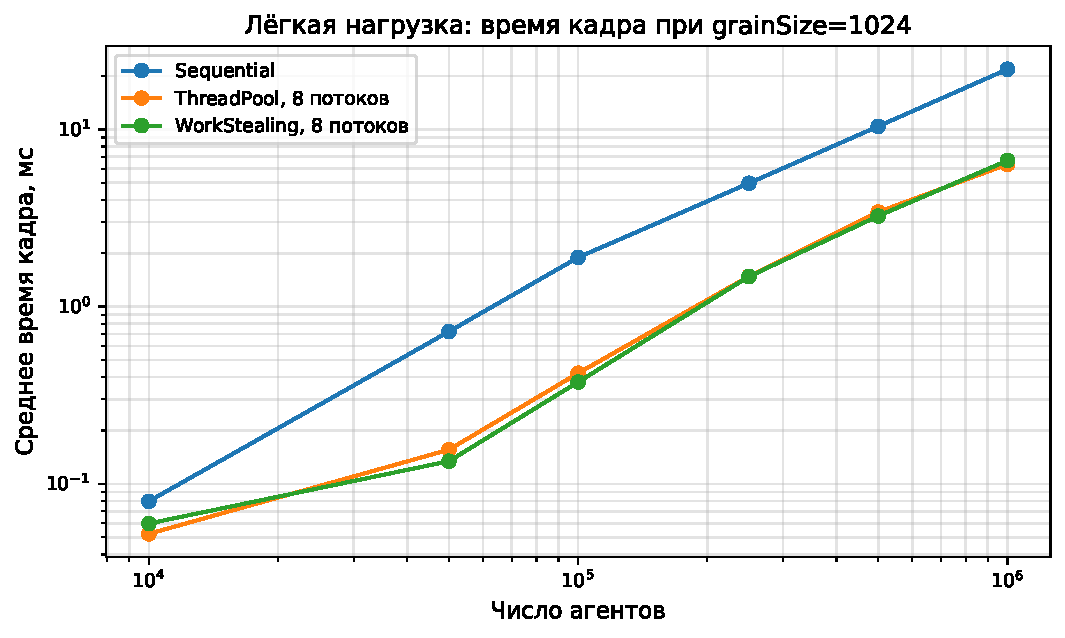
\includegraphics[width=0.84\textwidth]{figures/benchmarks/light_fixed_config_frame_by_agents.pdf}
\caption{Среднее время update-кадра на лёгкой нагрузке при \texttt{grainSize}=1024 и \(p=8\).}
\label{fig:light-fixed-frame-by-agents}
\end{figure}

При достаточно крупном размере задачи оба параллельных планировщика дают ускорение относительно \texttt{Sequential}. Однако результат зависит от размера входа: максимум ускорения достигается не всегда на самом большом \(N\). Это указывает на влияние расходов очередей, синхронизации и кэш-эффектов.

Ускорение для того же среза показано на рис.~\ref{fig:light-speedup-fixed}. Значения выше единицы означают выигрыш относительно последовательного обновления. В области \(N=50000\ldots100000\) ускорение достигает максимума, после чего не растёт монотонно. Это согласуется с тем, что рост числа агентов увеличивает полезную работу, но одновременно меняет поведение памяти, очередей и распределения задач.

\begin{figure}[ht]
\centering
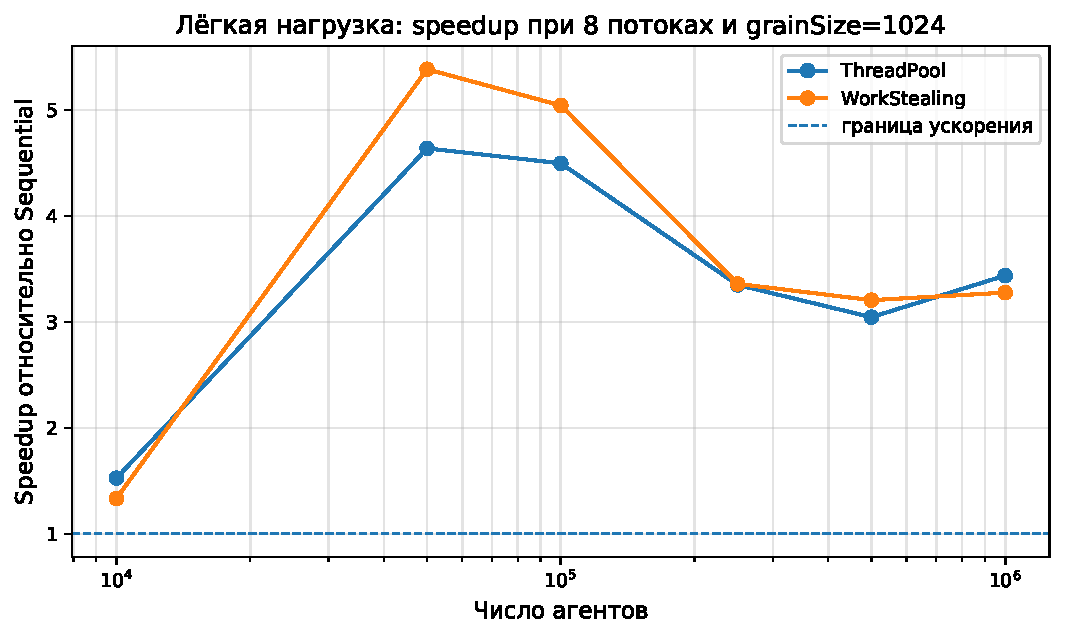
\includegraphics[width=0.84\textwidth]{figures/benchmarks/light_speedup_fixed_config_by_agents.pdf}
\caption{Ускорение относительно \texttt{Sequential} на лёгкой нагрузке при \(p=8\) и \texttt{grainSize}=1024.}
\label{fig:light-speedup-fixed}
\end{figure}

Показательный срез приведён в табл.~\ref{tab:light-best}. При \(N=50000\) и \(N=100000\) лучшим оказывается \texttt{WorkStealing}, но при \(N=10000\), \(N=500000\) и \(N=1000000\) минимальное время даёт \texttt{ThreadPool}. Следовательно, в равномерной лёгкой нагрузке нельзя заранее выбрать универсально лучший планировщик.

\begin{table}[ht]
\centering
\small
\caption{Лучшие парные конфигурации light-серии}
\label{tab:light-best}
\begin{tabular}{|r|r|r|r|r|r|c|}
\hline
\(N\) & \(p\) & \texttt{grainSize} & Seq, мс & TP, мс & WS, мс & Лучший \\
\hline
10000 & 8 & 1024 & 0{,}080 & 0{,}052 & 0{,}060 & TP \\
50000 & 8 & 1024 & 0{,}723 & 0{,}156 & 0{,}134 & WS \\
100000 & 8 & 1024 & 1{,}894 & 0{,}421 & 0{,}375 & WS \\
250000 & 8 & 4096 & 4{,}951 & 1{,}458 & 1{,}445 & WS \\
500000 & 8 & 4096 & 11{,}265 & 3{,}124 & 3{,}311 & TP \\
1000000 & 8 & 1024 & 21{,}827 & 6{,}348 & 6{,}661 & TP \\
\hline
\end{tabular}
\end{table}

\section{Относительное сравнение на лёгкой нагрузке}

Отдельный вопрос состоит в том, какой из двух параллельных планировщиков быстрее при одинаковом \texttt{grainSize}. На лёгкой нагрузке это сравнение не совпадает с вопросом об ускорении относительно \texttt{Sequential}. Возможна ситуация, где \texttt{WorkStealing} быстрее \texttt{ThreadPool}, но оба варианта проигрывают последовательному выполнению из-за слишком мелких задач.

На рис.~\ref{fig:light-ws-tp-ratio} показано отношение времени \texttt{ThreadPool} к времени \texttt{WorkStealing} при разных \texttt{grainSize}. Значения выше единицы означают, что \texttt{WorkStealing} быстрее. В полной light-серии он быстрее в 149 из 216 парных конфигураций. Особенно часто это происходит при малом \texttt{grainSize}, где локальные очереди могут снижать конкуренцию за общую очередь. Однако практический вывод по таким конфигурациям остаётся отрицательным, если они не дают ускорения относительно \texttt{Sequential}.

\begin{figure}[ht]
\centering
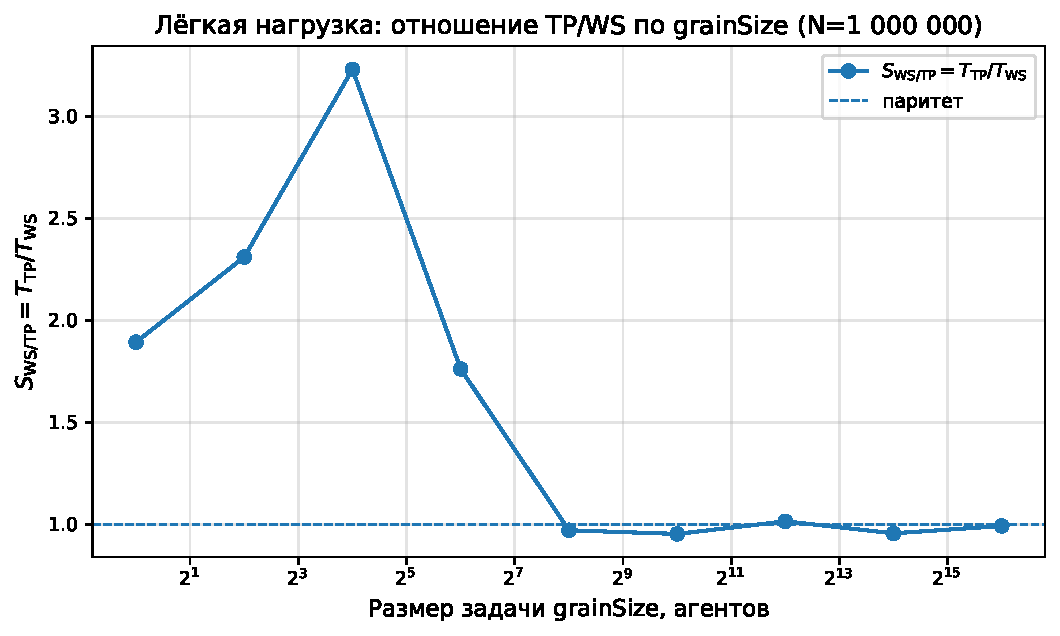
\includegraphics[width=0.84\textwidth]{figures/benchmarks/light_ws_tp_relative_by_grain.pdf}
\caption{Относительное сравнение \texttt{WorkStealing} и \texttt{ThreadPool} на лёгкой нагрузке.}
\label{fig:light-ws-tp-ratio}
\end{figure}

Таким образом, сравнение планировщиков следует выполнять в два этапа. Сначала нужно проверить, окупается ли само распараллеливание относительно последовательного обновления. Затем среди конфигураций, где ускорение действительно есть, можно выбирать более быстрый параллельный планировщик. Такой порядок защищает от ложного вывода, когда один параллельный вариант лучше другого, но оба непригодны для реального кадра.

\section{Влияние \texttt{grainSize}}

Размер задачи оказывает наибольшее влияние при лёгкой нагрузке. При \texttt{grainSize}=1 на \(N=1000000\) создаётся миллион задач, и расходы планирования доминируют над полезной работой. На рис.~\ref{fig:light-grain-large} показано, что увеличение \texttt{grainSize} резко снижает время кадра до области плато.

\begin{figure}[ht]
\centering
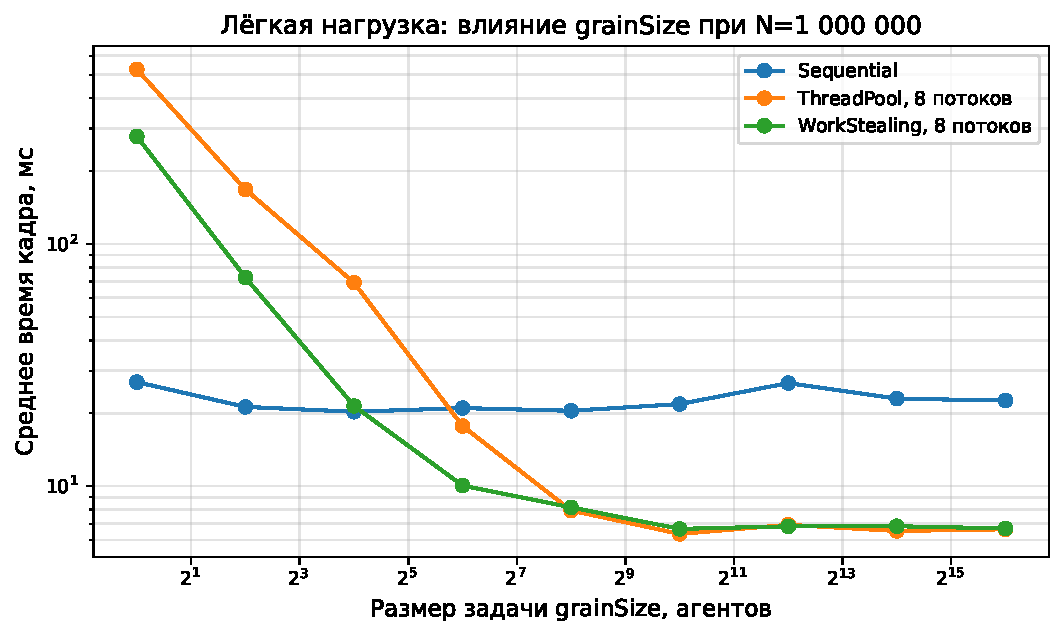
\includegraphics[width=0.84\textwidth]{figures/benchmarks/light_grain_effect_large_agents.pdf}
\caption{Влияние \texttt{grainSize} на среднее время кадра при лёгкой нагрузке, \(N=1000000\), \(p=8\).}
\label{fig:light-grain-large}
\end{figure}

При размере задачи 1 время \texttt{ThreadPool} равно \(526{,}732\) мс, а \texttt{WorkStealing} --- \(278{,}228\) мс. При размере 1024 эти значения уменьшаются до \(6{,}348\) и \(6{,}661\) мс соответственно. Значит, изменение только \texttt{grainSize} уменьшает время \texttt{ThreadPool} примерно в 83 раза, а \texttt{WorkStealing} --- примерно в 42 раза.

Относительный overhead показан на рис.~\ref{fig:light-fine-grain-overhead} и в табл.~\ref{tab:light-overhead}. При размере задачи 1 параллельные варианты значительно медленнее последовательного: \texttt{ThreadPool} проигрывает в \(19{,}58\) раза, а \texttt{WorkStealing} --- в \(10{,}34\) раза. При размере 16 \texttt{WorkStealing} находится около границы окупаемости, но \texttt{ThreadPool} всё ещё заметно медленнее. Начиная с \texttt{grainSize}=64 оба планировщика переходят в область полезного ускорения.

\begin{figure}[ht]
\centering
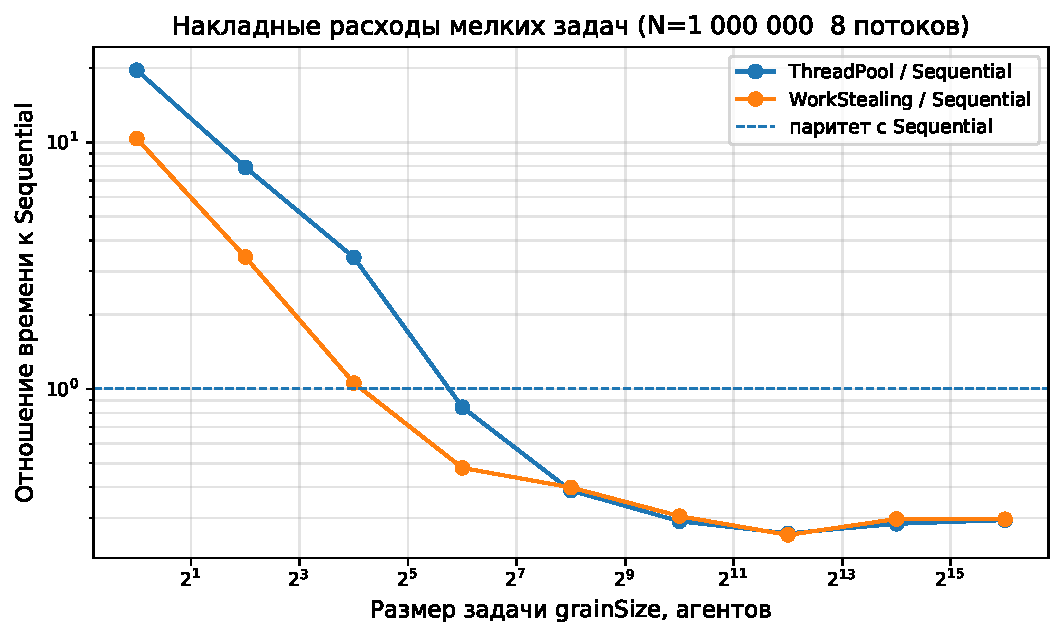
\includegraphics[width=0.84\textwidth]{figures/benchmarks/light_fine_grain_overhead.pdf}
\caption{Отношение времени параллельного выполнения к времени \texttt{Sequential} при \(N=1000000\), \(p=8\).}
\label{fig:light-fine-grain-overhead}
\end{figure}

\begin{table}[ht]
\centering
\small
\caption{Накладные расходы при \(N=1000000\), \(p=8\)}
\label{tab:light-overhead}
\begin{tabular}{|r|r|r|r|r|r|}
\hline
\texttt{grainSize} & Seq, мс & TP, мс & WS, мс & TP/Seq & WS/Seq \\
\hline
1 & 26{,}903 & 526{,}732 & 278{,}228 & 19{,}58 & 10{,}34 \\
4 & 21{,}248 & 168{,}066 & 72{,}761 & 7{,}91 & 3{,}42 \\
16 & 20{,}288 & 69{,}247 & 21{,}440 & 3{,}41 & 1{,}06 \\
64 & 21{,}008 & 17{,}708 & 10{,}052 & 0{,}84 & 0{,}48 \\
1024 & 21{,}827 & 6{,}348 & 6{,}661 & 0{,}29 & 0{,}31 \\
4096 & 26{,}655 & 6{,}925 & 6{,}825 & 0{,}26 & 0{,}26 \\
\hline
\end{tabular}
\end{table}

Инженерный вывод состоит в том, что для лёгких агентов микрозадачи непрактичны. Начиная примерно с \texttt{grainSize}=64, накладные расходы перестают полностью перекрывать пользу от параллелизма, но дальнейшее увеличение размера задачи не гарантирует монотонного улучшения.

\section{Тяжёлая неоднородная нагрузка}

В heavy-серии часть агентов выполняет дополнительную вычислительную ветку. На рис.~\ref{fig:heavy-ratio} показано, как среднее время кадра растёт с увеличением \texttt{HeavyRatio} при \(N=200000\), \(p=8\), \texttt{grainSize}=1024 и \texttt{HeavyIterations}=10000.

\begin{figure}[ht]
\centering
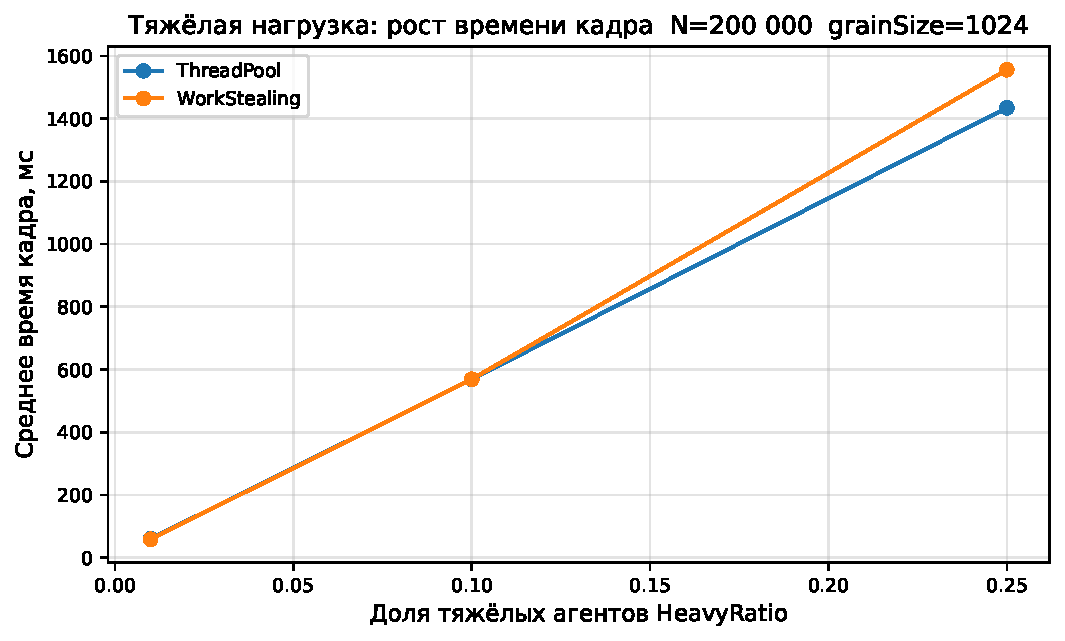
\includegraphics[width=0.84\textwidth]{figures/benchmarks/heavy_avg_frame_by_heavy_ratio.pdf}
\caption{Рост среднего времени кадра при увеличении доли тяжёлых агентов.}
\label{fig:heavy-ratio}
\end{figure}

Для \texttt{ThreadPool} время возрастает с \(60{,}240\) мс при \texttt{HeavyRatio}=0{,}01 до \(568{,}645\) мс при \texttt{HeavyRatio}=0{,}10 и \(1434{,}113\) мс при \texttt{HeavyRatio}=0{,}25. Для \texttt{WorkStealing} соответствующие значения равны \(58{,}530\), \(568{,}864\) и \(1555{,}543\) мс. Рост близок к росту объёма тяжёлой работы, что подтверждает пригодность модели heavy agents для управляемого создания нагрузки.

В лучших конфигурациях heavy-серии преимущество \texttt{WorkStealing} невелико и неустойчиво (табл.~\ref{tab:heavy-best}). При доле тяжёлых агентов \(0{,}25\) и 10000 итерациях лучший результат показывает \texttt{ThreadPool}. Это означает, что кража задач не гарантирует выигрыш даже при неоднородной нагрузке: её стоимость должна быть меньше стоимости простоя потоков.

\begin{table}[ht]
\centering
\small
\caption{Лучшие парные конфигурации heavy-серии при \(N=200000\)}
\label{tab:heavy-best}
\begin{tabular}{|r|r|r|r|r|r|c|}
\hline
\texttt{HeavyRatio} & \texttt{Iter.} & \(p\) & \texttt{grainSize} & TP, мс & WS, мс & Лучший \\
\hline
0{,}01 & 5000 & 8 & 1024 & 30{,}045 & 29{,}867 & WS \\
0{,}01 & 10000 & 8 & 64 & 58{,}429 & 57{,}607 & WS \\
0{,}10 & 5000 & 8 & 64 & 289{,}917 & 280{,}242 & WS \\
0{,}10 & 10000 & 8 & 64 & 564{,}045 & 576{,}804 & TP \\
0{,}25 & 5000 & 8 & 64 & 710{,}027 & 706{,}181 & WS \\
0{,}25 & 10000 & 8 & 64 & 1395{,}402 & 1485{,}887 & TP \\
\hline
\end{tabular}
\end{table}

\section{Стабильность времени кадра}

Среднее время кадра не всегда достаточно для оценки игровой системы. Если среднее значение приемлемо, но отдельные кадры имеют большой максимум, игрок всё равно увидит рывки. Поэтому в heavy-серии дополнительно рассматривались \texttt{MinFrameMs} и \texttt{MaxFrameMs}.

На рис.~\ref{fig:heavy-min-max-stability} видно, что с ростом доли тяжёлых агентов увеличивается не только среднее время, но и разброс между лучшими и худшими кадрами. Это ожидаемо: чем больше дорогих агентов попадает в задачи, тем выше вероятность неравномерного распределения работы между потоками. Для game loop это означает, что планировщик должен оцениваться не только по \texttt{AvgFrameMs}, но и по худшим кадрам.

\begin{figure}[ht]
\centering
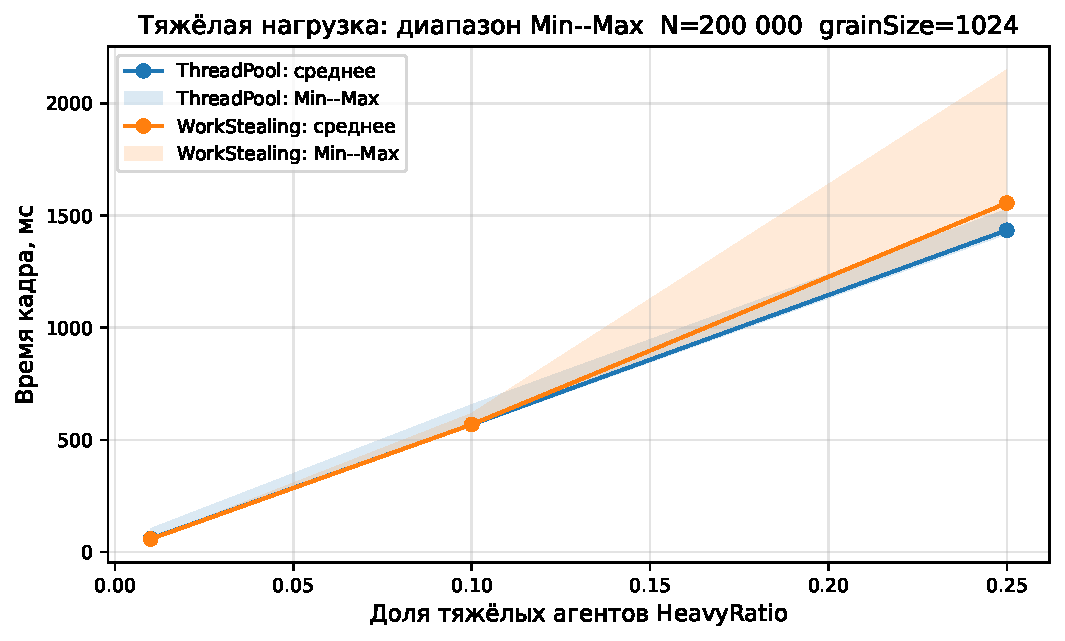
\includegraphics[width=0.84\textwidth]{figures/benchmarks/heavy_min_max_stability.pdf}
\caption{Минимальное, среднее и максимальное время кадра в тяжёлой серии.}
\label{fig:heavy-min-max-stability}
\end{figure}

Дополнительная нормированная метрика показана на рис.~\ref{fig:heavy-relative-range}. Она отражает относительный размах между минимальным и максимальным временем кадра. Такая нормировка удобна, потому что при росте \texttt{HeavyRatio} абсолютные времена увеличиваются на порядок, и прямое сравнение миллисекунд хуже показывает стабильность.

\begin{figure}[ht]
\centering
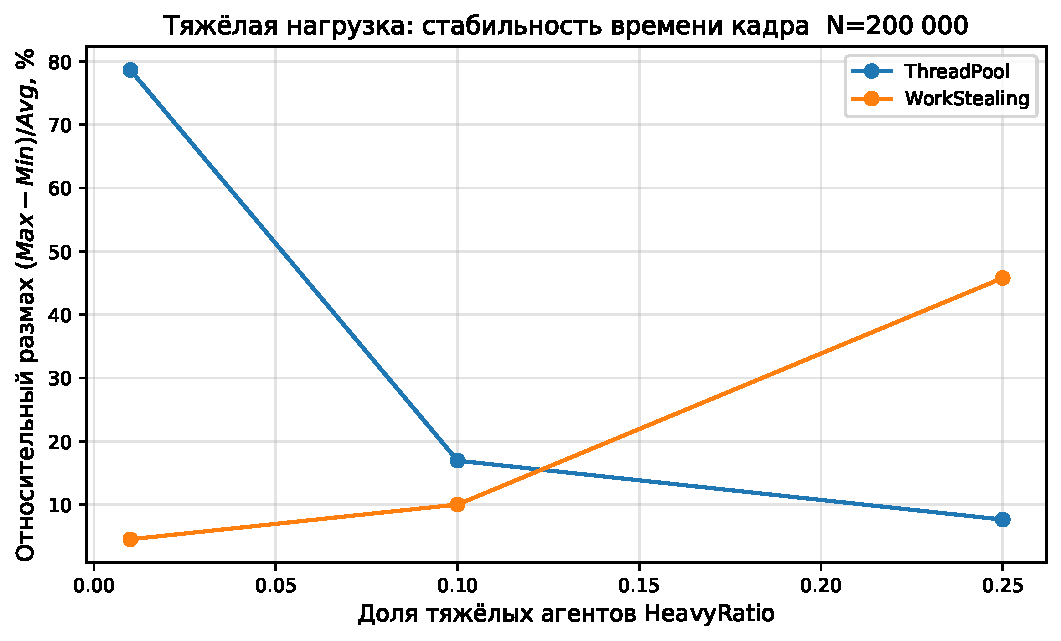
\includegraphics[width=0.84\textwidth]{figures/benchmarks/heavy_relative_range_by_heavy_ratio.pdf}
\caption{Нормированный разброс времени кадра при разной доле тяжёлых агентов.}
\label{fig:heavy-relative-range}
\end{figure}

В ряде срезов \texttt{WorkStealing} уменьшает худший кадр, но этот эффект также не является гарантированным. При высокой доле heavy agents стоимость кражи и локальная структура распределения задач могут привести к тому, что простой \texttt{ThreadPool} окажется стабильнее. Поэтому для практического применения нужно смотреть на распределение времени кадров, а не только на среднее значение.

\section{Размер задачи при тяжёлой нагрузке}

При тяжёлой нагрузке оптимальный \texttt{grainSize} может быть меньше, чем в light-сценарии. Причина в том, что каждая задача содержит больше полезной работы, а значит, дополнительные задачи не так сильно увеличивают относительный overhead. При этом меньшие блоки улучшают балансировку тяжёлых агентов между потоками.

На рис.~\ref{fig:heavy-grain-effect} показано влияние \texttt{grainSize} на тяжёлую серию. Для части конфигураций лучший результат достигается при \texttt{grainSize}=64 или 256, то есть при более мелком разбиении, чем в лёгкой нагрузке. Это подчёркивает, что универсального размера блока нет: параметр должен подбираться под конкретную стоимость агента и распределение тяжёлой работы.

\begin{figure}[ht]
\centering
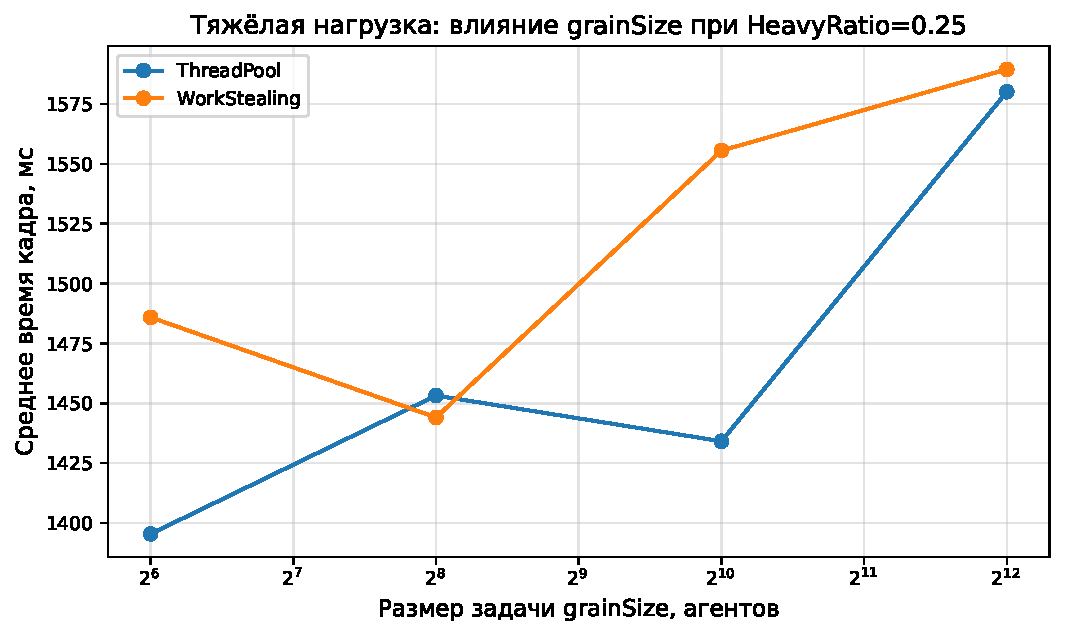
\includegraphics[width=0.84\textwidth]{figures/benchmarks/heavy_grain_effect.pdf}
\caption{Влияние \texttt{grainSize} на среднее время кадра при тяжёлой нагрузке.}
\label{fig:heavy-grain-effect}
\end{figure}

\section{Масштабирование и сравнение планировщиков}

При тяжёлой нагрузке полезная работа велика, поэтому относительная доля scheduling overhead уменьшается. На рис.~\ref{fig:heavy-scaling} показан переход с 4 на 8 потоков. В рассмотренных срезах ускорение близко к двукратному: примерно \(1{,}87\)--\(1{,}94\) для \texttt{ThreadPool} и \(1{,}81\)--\(1{,}95\) для \texttt{WorkStealing}. Это подтверждает, что многопоточность наиболее полезна, когда задача содержит достаточно вычислений.

\begin{figure}[ht]
\centering
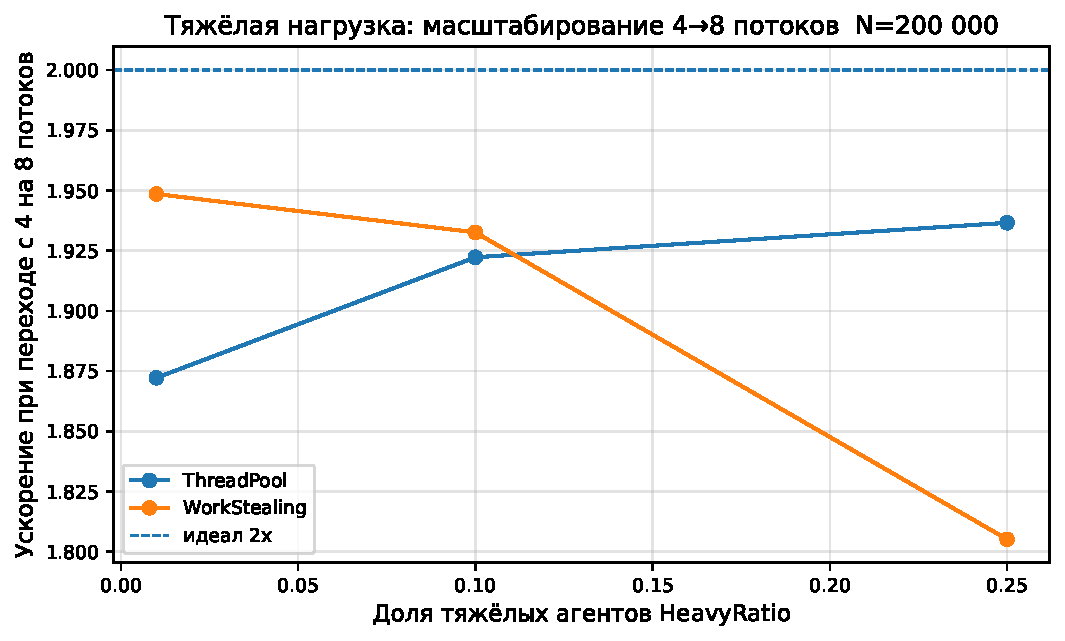
\includegraphics[width=0.84\textwidth]{figures/benchmarks/heavy_scaling_4_to_8.pdf}
\caption{Масштабирование тяжёлой нагрузки при переходе с 4 на 8 потоков.}
\label{fig:heavy-scaling}
\end{figure}

Сравнение \texttt{ThreadPool} и \texttt{WorkStealing} показало отсутствие универсального победителя. В light-серии \texttt{WorkStealing} быстрее в 149 из 216 парных конфигураций, то есть в \(69{,}0\%\) пар, но при слишком малом \texttt{grainSize} обе реализации могут быть медленнее \texttt{Sequential}. В heavy-серии \texttt{ThreadPool} быстрее в 110 из 192 пар, а \texttt{WorkStealing} --- в 82 из 192.

На рис.~\ref{fig:heavy-ws-tp} приведено относительное сравнение двух параллельных планировщиков в тяжёлой серии. Значения около единицы означают близкую производительность. Видно, что при некоторых параметрах \texttt{WorkStealing} выигрывает, но при других уступает. Это особенно важно для инженерной интерпретации: наличие механизма stealing не гарантирует лучшего результата, если исходное разбиение уже достаточно сбалансировано или если steal-операции создают заметные расходы.

\begin{figure}[ht]
\centering
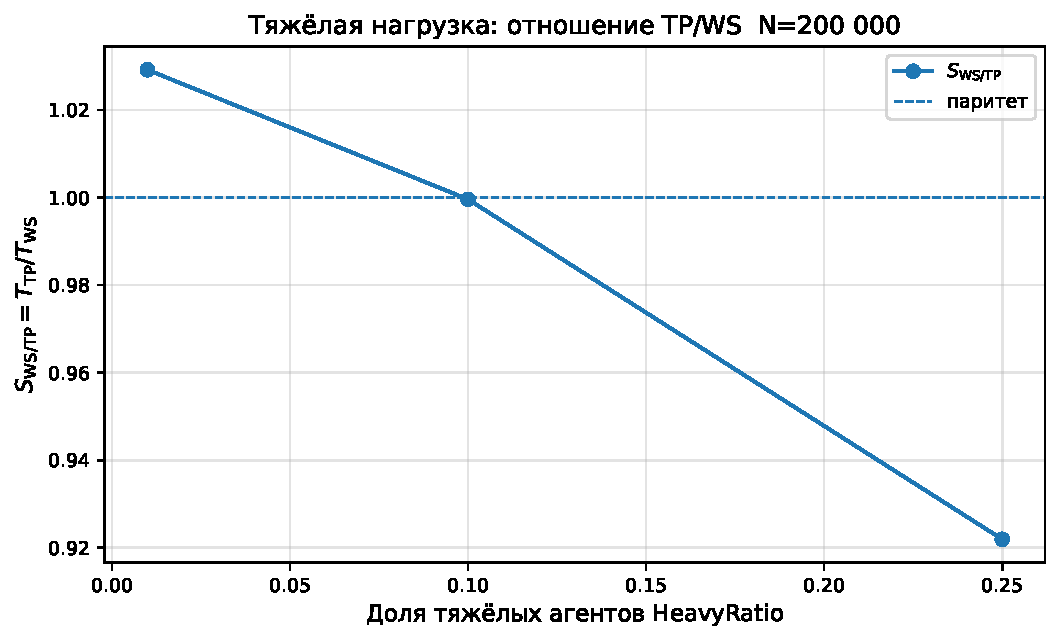
\includegraphics[width=0.84\textwidth]{figures/benchmarks/heavy_ws_tp_relative_speedup.pdf}
\caption{Относительное сравнение \texttt{WorkStealing} и \texttt{ThreadPool} в тяжёлой серии.}
\label{fig:heavy-ws-tp}
\end{figure}

Следовательно, work stealing следует рассматривать как инструмент для определённых типов дисбаланса, а не как безусловно более производительный планировщик. Если задачи однородны или стоимость stealing сравнима с выигрышем от балансировки, простой пул потоков может быть не хуже.

Полученные результаты также согласуются с законом Амдала. Если в кадре остаётся значительная последовательная часть или если планировщик добавляет существенные служебные расходы, увеличение числа потоков не даёт пропорционального ускорения. В light-серии это проявляется особенно явно: сама полезная работа мала, поэтому даже восемь потоков не помогают при слишком мелком \texttt{grainSize}. В heavy-серии полезная часть больше, и масштабирование между 4 и 8 потоками становится ближе к идеальному, хотя всё равно ограничивается балансировкой и overhead.

С инженерной точки зрения это означает, что оптимизация должна начинаться не с выбора «самого сложного» планировщика, а с анализа структуры работы. Если update агента занимает мало времени, выгоднее укрупнять блоки, улучшать layout данных и уменьшать синхронизацию. Если же агент дорогой и неоднородный, на первый план выходят балансировка и контроль худших кадров.

\section{Практические рекомендации и ограничения}

По результатам экспериментов можно выделить несколько рекомендаций. Во-первых, не следует распараллеливать слишком мелкие операции без группировки в задачи достаточного размера. Во-вторых, \texttt{grainSize} необходимо подбирать экспериментально, потому что оптимум зависит от числа агентов, числа потоков, стоимости агента и реализации очередей. В-третьих, \texttt{ThreadPool} подходит для равномерной нагрузки и хорошо выбранного разбиения. В-четвёртых, \texttt{WorkStealing} целесообразен при выраженном дисбалансе, но его преимущество должно подтверждаться benchmark-ом.

\begin{table}[ht]
\centering
\small
\caption{Сводные рекомендации по выбору параметров}
\label{tab:recommendations}
\begin{tabularx}{\textwidth}{|p{0.30\textwidth}|X|}
\hline
Ситуация & Практическое решение \\
\hline
Лёгкие однотипные агенты & Увеличивать \texttt{grainSize} до области, где overhead перестаёт доминировать; сначала сравнивать с \texttt{Sequential}. \\
\hline
Тяжёлые агенты & Использовать несколько потоков; проверять масштабирование между 4 и 8 потоками и не выбирать слишком крупные блоки. \\
\hline
Неоднородная стоимость задач & Проверять \texttt{WorkStealing} в парном сравнении, но не считать его выигрыш гарантированным. \\
\hline
Требование стабильного кадра & Смотреть не только на \texttt{AvgFrameMs}, но и на \texttt{MaxFrameMs} и относительный разброс. \\
\hline
Перенос в игровой движок & Повторять benchmark на реальной логике агентов, с фактическим layout-ом данных и зависимостями между подсистемами. \\
\hline
\end{tabularx}
\end{table}

Работа имеет ограничения. Модель агента упрощена и не включает полноценную физику, анимацию, навигацию, сетевую синхронизацию и межагентные зависимости. Реализация \texttt{WorkStealing} является исследовательской, а не production-grade job system. Кроме того, результаты зависят от аппаратной платформы, компилятора и флагов оптимизации. Поэтому численные значения нельзя переносить в другие движки напрямую; основную ценность имеют выявленные закономерности.

\section{Выводы по главе}

Эксперименты подтвердили, что размер задачи является ключевым фактором производительности. В light-сценарии чрезмерно мелкий \texttt{grainSize} делает параллельное выполнение значительно медленнее последовательного. В heavy-сценарии масштабирование лучше, потому что полезная работа перекрывает служебные расходы. При этом \texttt{ThreadPool} и \texttt{WorkStealing} требуют парного сравнения: ни один из них не оказался универсально лучшим.
\newpage
\section*{Заключение}
\addcontentsline{toc}{chapter}{Заключение}

В работе исследовано применение многопоточности к массовому обновлению игровых ИИ-агентов. Теоретический анализ показал, что такая нагрузка естественно выражается как параллельный проход по массиву данных, но корректность и эффективность требуют дисциплины доступа к состоянию мира, разделения параллельных и синхронизационных фаз, а также контроля накладных расходов.

В практической части разработана экспериментальная система задач с единым интерфейсом \texttt{IScheduler}. Реализованы три стратегии выполнения: \texttt{Sequential}, \texttt{ThreadPool} и \texttt{WorkStealing}. Для оценки производительности проведены серии бенчмарков с разным числом агентов, потоков, размером задач и долей тяжёлых агентов.

Главный результат состоит в том, что многопоточность эффективна только при достаточном объёме полезной работы на задачу. При лёгкой нагрузке и \texttt{grainSize}=1 планировщик \texttt{ThreadPool} оказался медленнее \texttt{Sequential} в \(19{,}58\) раза, а \texttt{WorkStealing} --- в \(10{,}34\) раза. При увеличении \texttt{grainSize} накладные расходы уменьшаются, и параллельное выполнение начинает давать выигрыш.

Для тяжёлой нагрузки переход с 4 на 8 потоков даёт почти двукратное ускорение в показательных сценариях. Однако сравнение \texttt{ThreadPool} и \texttt{WorkStealing} не выявило универсального лидера: в heavy-серии \texttt{ThreadPool} быстрее в 110 из 192 парных конфигураций, а \texttt{WorkStealing} --- в 82 из 192. Это подтверждает, что выбор планировщика должен основываться на измерениях.

Практический вывод работы заключается в необходимости benchmark-driven подхода к многопоточному ИИ. Нельзя заранее считать, что больше потоков, меньшие задачи или более сложный планировщик дадут лучший результат. Эффективность определяется сочетанием архитектуры данных, \texttt{grainSize}, характера нагрузки и стоимости планирования.

Дальнейшее развитие работы может идти в нескольких направлениях. Во-первых, модель агента можно усложнить за счёт навигационных запросов, сенсорики и межагентных зависимостей. Во-вторых, полезно сравнить array-of-structures и structure-of-arrays layout, поскольку кэш-локальность существенно влияет на массовые проходы. В-третьих, можно добавить граф зависимостей задач и отдельную commit-фазу, чтобы приблизить прототип к production job system. Такие расширения позволят проверить, сохраняются ли найденные закономерности в более реалистичной игровой архитектуре.

\begin{thebibliography}{99}

\bibitem{unity_job_system}
Unity Technologies.
\textit{Job system overview}.
Unity Manual.
URL: \url{https://docs.unity3d.com/6000.2/Documentation/Manual/job-system-overview.html}

\bibitem{unity_parallel_for_jobs}
Unity Technologies.
\textit{ParallelFor jobs}.
Unity Manual.
URL: \url{https://docs.unity3d.com/2020.1/Documentation/Manual/JobSystemParallelForJobs.html}

\bibitem{unity_ijobparallelfor}
Unity Technologies.
\textit{IJobParallelFor}.
Unity Scripting API.
URL: \url{https://docs.unity3d.com/ScriptReference/Unity.Jobs.IJobParallelFor.html}

\bibitem{unity_safety_system}
Unity Technologies.
\textit{The safety system in the C\# Job System}.
Unity Manual.
URL: \url{https://docs.unity3d.com/2020.1/Documentation/Manual/JobSystemSafetySystem.html}

\bibitem{unreal_tasks_system}
Epic Games.
\textit{Tasks Systems in Unreal Engine}.
Unreal Engine Documentation.
URL: \url{https://dev.epicgames.com/documentation/unreal-engine/tasks-systems-in-unreal-engine}

\bibitem{unreal_task_graph_insights}
Epic Games.
\textit{Task Graph Insights in Unreal Engine 5}.
Unreal Engine Documentation.
URL: \url{https://dev.epicgames.com/documentation/unreal-engine/task-graph-insights-in-unreal-engine-5}

\bibitem{gdc_naughty_fibers}
Gyrling, C.
\textit{Parallelizing the Naughty Dog Engine Using Fibers}.
Game Developers Conference, 2015.
URL: \url{https://www.gdcvault.com/play/1022186/parallelizing-the-naughty-dog-engine}

\bibitem{gdc_task_based_multithreading}
Game Developers Conference.
\textit{Task-based Multithreading: How to Program for 100 cores}.
GDC Vault.
URL: \url{https://gdcvault.com/play/1012321/Task-based-Multithreading-How-to}

\bibitem{onetbb_scheduler}
Intel.
\textit{How Task Scheduler Works}.
Intel oneAPI Threading Building Blocks Documentation.
URL: \url{https://www.intel.com/content/www/us/en/docs/onetbb/developer-guide-api-reference/2021-6/how-task-scheduler-works.html}

\bibitem{onetbb_parallel_for}
Intel.
\textit{parallel\_for}.
Intel oneAPI Threading Building Blocks Documentation.
URL: \url{https://www.intel.com/content/www/us/en/docs/onetbb/developer-guide-api-reference/2021-9/parallel-for.html}

\bibitem{ms_thread_pool}
Microsoft.
\textit{Thread Pools}.
Win32 Apps Documentation.
URL: \url{https://learn.microsoft.com/en-us/windows/win32/procthread/thread-pools}

\bibitem{amdahl_1967}
Amdahl, G. M.
\textit{Validity of the Single Processor Approach to Achieving Large Scale Computing Capabilities}.
AFIPS Conference Proceedings, 30, 483--485, 1967.
URL: \url{https://www3.cs.stonybrook.edu/~rezaul/Spring-2012/CSE613/reading/Amdahl-1967.pdf}

\end{thebibliography}

\end{document}
